% QDPT Springer Nature working source.
% This file keeps modular inputs for editing. Generate qdpt-sn.tex as the single-file submission copy.
\documentclass[pdflatex,sn-mathphys-num]{sn-jnl}

\usepackage[UTF8,scheme=plain]{ctex}
\usepackage{graphicx}
\usepackage{amsmath,amssymb,amsfonts}
\usepackage{booktabs}
\usepackage{float}
\usepackage{xcolor}

\raggedbottom

\begin{document}

\title[Question-Guided Directional Prompting]{Question-Guided Directional Prompting for Parameter-Efficient Domain Adaptation of Frozen Multimodal Large Language Models}

% 待补：按投稿系统中的顺序填写作者、通信作者、邮箱和单位。
% \author*[1]{\fnm{Given Name} \sur{Family Name}}\email{address@example.com}
% \affil*[1]{\orgdiv{Department}, \orgname{University}, \orgaddress{\city{City}, \country{Country}}}

\abstract{We present Question-Guided Directional Prompt Tuning (QDPT) for adapting frozen multimodal large language models to specialized visual domains. QDPT pools question token embeddings into queries, reads intermediate visual features through cross-attention, and maps the aggregated evidence to dynamic language prompts. On Qwen3-VL-4B-Instruct, QDPT trains 7.81 million parameters while retaining the original backbone weights. On PathVQA, QDPT achieves 58.88\% test accuracy, improving over static language prompts and a CoCoOp-style baseline by 2.80 and 1.93 percentage points, respectively, while remaining 0.78 points below full-attention LoRA-r8. Ablations show a modest, seed-dependent benefit from question conditioning and support the contribution of the visual branch. In a controlled 100-step training benchmark, QDPT achieves 1.88$\times$ the throughput of full-attention LoRA-r8 with 18.2\% lower peak allocated GPU memory. QDPT reaches 76.95\% on SLAKE and 71.38\% on a private electrical inspection test.}

\keywords{multimodal large language models, parameter-efficient fine-tuning, dynamic prompt tuning, visual question answering, domain adaptation}

\maketitle

\section{引言}

多模态大语言模型能够接收图像与文本输入，以生成方式完成视觉问答和多轮交互\cite{Alayrac2022FlamingoAV,li2023blip,Liu2023VisualIT,Zhu2023MiniGPT4EV,Bai2025Qwen3VLTR}。将通用模型用于专业场景时，新的图像分布、术语和任务要求通常需要进一步适配，例如医学图像判读和电力设备巡检\cite{He2020PathVQA3Q,Liu2021SlakeAS,Wang2024PowerLLaVALL}。同一设备图像可能对应部件识别、连接关系或异常位置等不同问题，回答所需的视觉线索也随之改变。完整微调需要更新并保存整套模型权重，多领域部署因此面临较高的训练与存储成本\cite{houlsby2019parameter,Hu2022LoRA}。

参数高效微调通过少量可训练参数完成适配。LoRA、IA$^3$和AdaLoRA分别通过低秩更新、激活缩放和自适应预算分配调整网络内部变换\cite{Hu2022LoRA,Liu2022FewShotPF,Zhang2023AdaLoRAAB}。Prompt Tuning及其深层扩展则学习连续上下文，引导冻结模型完成下游任务\cite{li2021prefix,lester2021power,Liu2021PTuningVP,jia2022visual}。静态Prompt在样本间共享，适合学习常见的任务模式；视觉问答还需要利用当前问题确定相关对象和属性\cite{dai2023instructblip}。

条件Prompt和视觉聚合为这种样本差异提供了处理方式。在CLIP的图文表示空间中，CoOp学习共享上下文，CoCoOp进一步引入图像条件Token，MaPLe则联合调整视觉与语言Prompt\cite{Radford2021LearningTV,Zhou2021LearningTP,Zhou2022ConditionalPL,Khattak2022MaPLeMP}。少量潜在Token也可用于汇聚视觉输入\cite{Jaegle2021PerceiverGP,Ryoo2021TokenLearnerWC}：BLIP-2通过Q-Former连接冻结视觉编码器与语言模型，InstructBLIP让指令参与视觉提取，DRAPE则根据指令与视觉特征生成动态Soft Prompt\cite{li2023blip,dai2023instructblip,Hu2026DynamicCP}。本文考察一种具体的领域适配结构：从视觉编码器中间层读取问题相关特征，将其映射为语言侧动态Prompt，并保留共享的静态Prompt。

我们提出Question-Guided Directional Prompt Tuning（QDPT）。该方法对问题Token嵌入进行注意力池化，以所得Query读取视觉编码器中间层特征，并将聚合结果转换为10个语言Prompt。视觉编码器、Merger和语言模型的原有参数在训练中保持固定；适配器还包含视觉侧与语言侧的连续Prompt。各类输入在自回归语言模型中的排列通过Validation实验确定。

实验在PathVQA、SLAKE和自建电气数据集上比较QDPT与静态Prompt、图像条件Prompt及LoRA。在PathVQA Test上，QDPT较静态语言Prompt和CoCoOp-style分别提高2.80和1.93个百分点，较LoRA低0.78个百分点。三次Learned Query对照显示，问题条件Query的平均准确率高0.83个百分点，但这一优势没有在所有种子中复现。统一条件下的短程训练测试中，QDPT的吞吐为LoRA的1.88倍，峰值分配显存低18.18\%。本文的工作包括：

\begin{itemize}
    \item 构建面向冻结生成式MLLM的Prompt适配器，用当前问题读取视觉编码器中间层特征，并将聚合结果转换为语言侧动态Prompt。
    \item 通过可训练参数量匹配的Learned Query、关闭视觉Cross-Attention和移除静态视觉Prompt等对照分析各分支；公开VQA基准报告多随机种子结果，电气数据用于单次应用验证。
\end{itemize}

\section{相关工作}

\subsection{多模态大模型的参数高效适配}

将大模型迁移到多个下游任务时，完整微调带来的训练开销和独立权重存储需求促使研究者缩小参数更新范围。在语言模型中，Adapter通过插入小型瓶颈模块学习任务相关变换\cite{houlsby2019parameter}，LoRA进一步以低秩矩阵表示权重增量\cite{Hu2022LoRA}。围绕适配预算的分配，IA$^3$将更新限制为激活上的缩放向量\cite{Liu2022FewShotPF}，AdaLoRA则在训练中调整各模块的低秩预算\cite{Zhang2023AdaLoRAAB}。这些方法通过少量参数改变网络内部的特征变换，为领域适配提供了较直接的优化空间。

另一类方法通过学习连续上下文引导冻结模型完成下游任务。Prompt Tuning在输入侧优化少量Token\cite{lester2021power}，Prefix Tuning和P-Tuning v2将可训练上下文引入更深的Transformer计算，以提高Prompt对模型输出的影响\cite{li2021prefix,Liu2021PTuningVP}。当适配对象扩展到视觉和视觉语言模型时，新的问题是如何同时调整图像表示及其与语言的对应关系。Visual Prompt Tuning在视觉编码器内加入连续Token\cite{jia2022visual}，VL-Adapter研究视觉语言任务中的轻量模块适配\cite{sung2021vl}，MaPLe则通过耦合视觉与语言Prompt协调两种模态的更新\cite{Khattak2022MaPLeMP}。多模态PEFT的实证研究也表明，适配模块的位置会影响任务性能与计算成本\cite{zhou2024empirical}。由此，适配设计需要同时考虑参数预算、作用位置和输入样本之间的差异。

\subsection{条件Prompt与问题引导的视觉聚合}

样本共享的Prompt能够学习领域中的常见模式，但同一领域内的图像和问题仍有不同的证据需求。视觉语言分类首先从实例条件化的角度处理这一问题：在CLIP建立的图文表示空间中\cite{Radford2021LearningTV}，CoOp学习任务共享的连续上下文\cite{Zhou2021LearningTP}，CoCoOp针对固定上下文对训练类别的过拟合，引入由图像特征生成的条件Token\cite{Zhou2022ConditionalPL}。从分类扩展到生成式问答后，条件信息还包括用户提出的问题，视觉聚合也需要随问题所关注的对象和属性改变。

实现这种聚合需要将较长的视觉序列转换为少量有用表示。Perceiver通过潜在向量与输入之间的Cross-Attention处理高维数据\cite{Jaegle2021PerceiverGP}，TokenLearner通过自适应空间聚合减少视觉Token数量\cite{Ryoo2021TokenLearnerWC}。在冻结视觉编码器与语言模型的连接处，BLIP-2用Q-Former的可学习Query提取固定长度的视觉表示\cite{li2023blip}；InstructBLIP进一步引入指令，使视觉提取过程围绕当前任务展开\cite{dai2023instructblip}。这一发展将视觉压缩与任务条件化联系起来，也为从现有MLLM中读取问题相关证据提供了结构基础。

近期工作进一步将条件视觉聚合用于轻量适配。DRAPE根据指令构造Query，从视觉特征中生成实例级Soft Prompt；它面向持续指令学习，训练共享视觉投影，并借助任务路由和零空间约束处理任务序列\cite{Hu2026DynamicCP}。GRASP则针对遥感图像划分空间区域，根据问题表示稀疏组合区域Prompt原型\cite{Sun2026GRASPGR}。QDPT采用相近的“文本Query读取视觉K/V”组件，但研究对象和冻结边界不同：视觉编码器、Merger与LLM均保持固定，Query读取视觉编码器中间层特征，所得表示与静态领域Prompt共同接入语言模型。Query--K/V沿用标准Cross-Attention，本文考察的是这套组织方式在冻结生成式MLLM中的适配效果、分支作用和训练代价。

\subsection{专业视觉领域中的多模态模型}

专业视觉任务将上述适配问题落实为具体的图像判读和回答需求。在医学领域，PathVQA与SLAKE提供了组织、病变及相关知识的问答数据，使模型能够在开放式与封闭式问题上接受评价\cite{He2020PathVQA3Q,Liu2021SlakeAS}。针对回答缺少区域依据的问题，CoTBox-TTT利用视觉思维链框定位相关区域，并在测试阶段优化Evidence Prompt与Answer Prompt\cite{Qian2025CoTBoxTTTGM}。其适配发生在单个测试样本上；本文则在领域训练集上学习Prompt生成器，推理时通过一次前向计算生成样本相关的上下文。

设备巡检同样要求把局部视觉线索转化为专业判断，但关注对象转为设备部件、缺陷和运行状态。Power-LLaVA围绕输电线路巡检构建视觉语言助手\cite{Wang2024PowerLLaVALL}，电网资产检查研究进一步考察多模态模型在实际运维任务中的识别与解释能力\cite{Rocha2025AdvancesIE,Hao2025PowerGI}。在训练样本有限或故障类型存在差异时，DefectGPT研究有限电气样本下的多类别缺陷检测\cite{lin2025defectgpt}，光伏故障诊断工作则通过动态LoRA路由进行领域适配\cite{Wu2026DomainAdaptiveML}。这些研究说明了专业任务对适配方法的具体要求：模型既要识别图像中的设备与状态，也要按问题组织领域相关的回答。本文据此在公开VQA基准上比较适配结构，并用自建电力电气数据集补充应用验证。

\section{方法}
\label{sec:method}

\subsection{基础模型与总体结构}

本文以Qwen3-VL-4B-Instruct\cite{Bai2025Qwen3VLTR}为基础模型，记为$F_{\Phi}$，其中$\Phi$包含视觉编码器、视觉Merger、词嵌入层和自回归语言模型的参数。模型接收图像$I$和问题文本$X$，生成答案$Y$。领域训练集记为$\mathcal{D}=\{(I_i,X_i,Y_i)\}_{i=1}^{N}$。QDPT在基础模型中加入参数为$\Theta$的Prompt适配器，固定$\Phi$，通过答案Token上的自回归负对数似然优化$\Theta$：

\begin{equation}
\mathcal{L}(\Theta)
=-\sum_{i=1}^{N}\sum_{t=1}^{|Y_i|}
\log p_{\Phi,\Theta}
\left(y_{i,t}\mid I_i,X_i,Y_{i,<t}\right),
\qquad \Phi\ \text{保持冻结}.
\end{equation}

训练时，梯度通过冻结层传回适配器，使Prompt能够调整后续Token的表示。

图\ref{fig:qdpt-global}展示从图像和问题输入到答案生成的整体流程。

\begin{figure}[t]
    \centering
    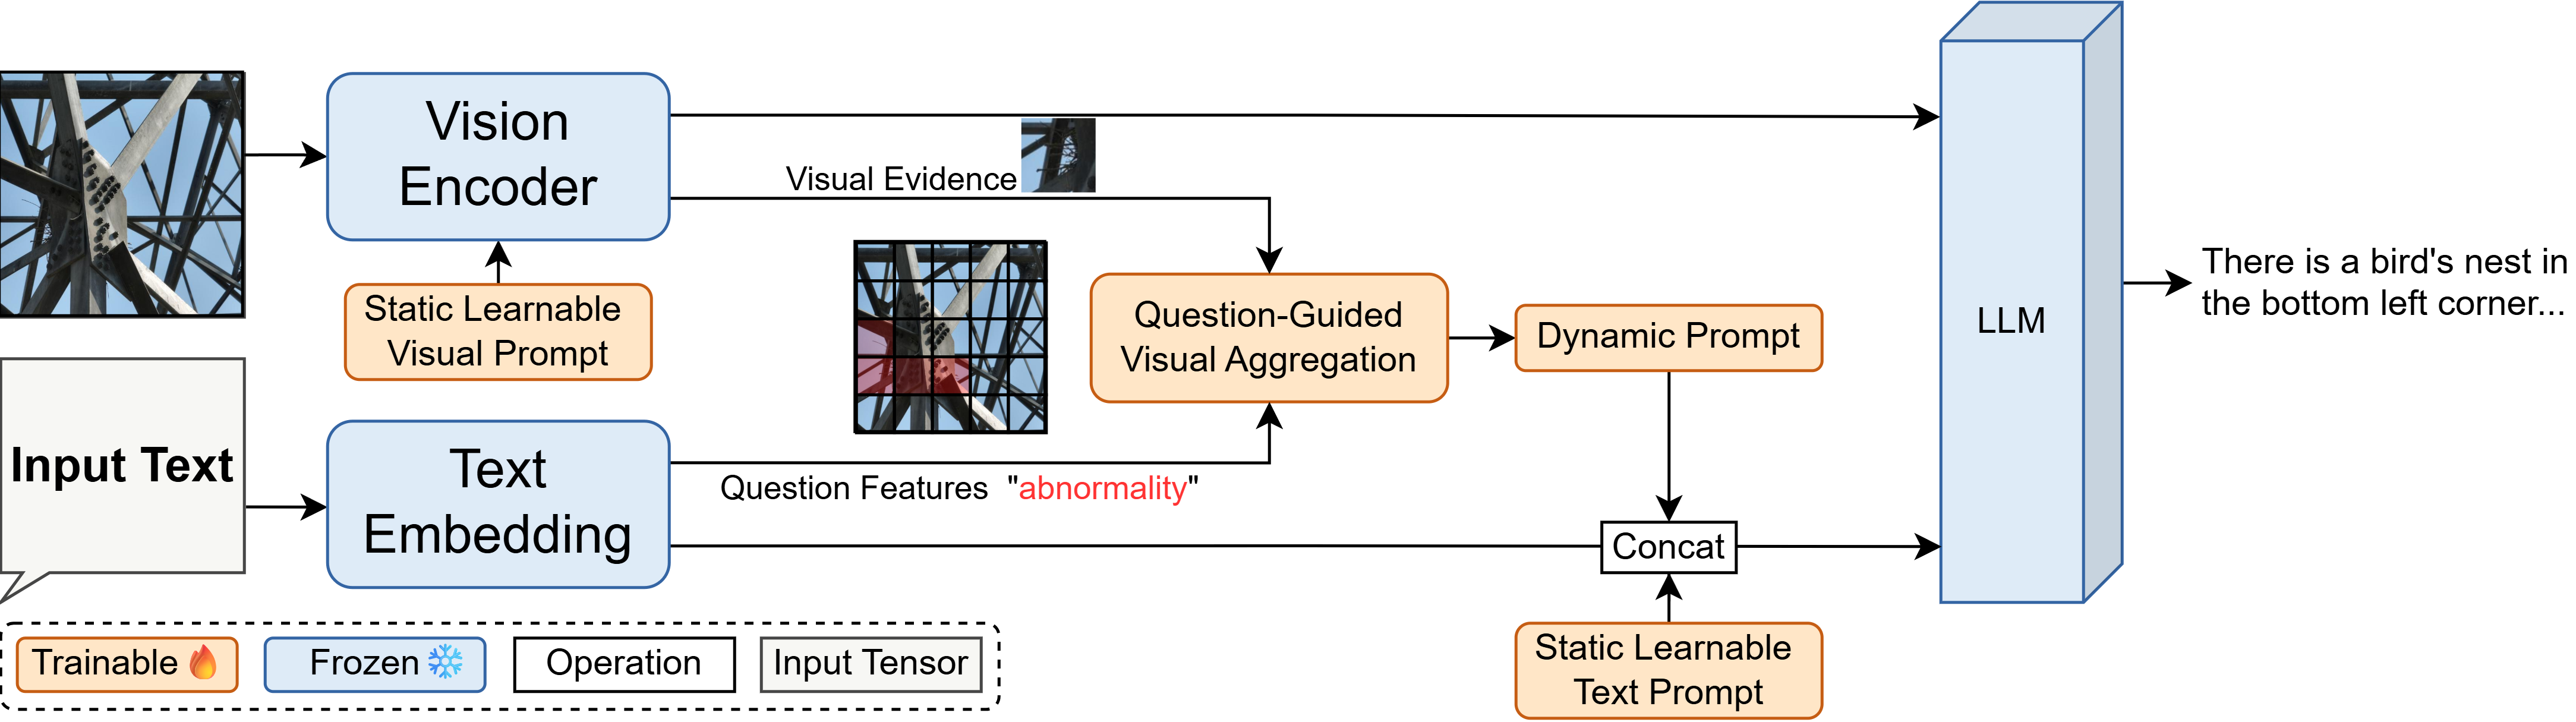
\includegraphics[width=\textwidth]{figures/qdpt_global_overview.png}
    \caption{QDPT整体框架。问题引导的视觉聚合生成样本相关的动态Prompt，静态Prompt在视觉侧与语言侧提供领域校准。蓝色模块的原有参数保持冻结，橙色模块为适配部分；视觉区域与问题关键词用于示意证据选择。}
    \label{fig:qdpt-global}
\end{figure}

视觉编码器包含24层Transformer，隐藏维度$d_v=1024$；语言模型包含36层Transformer，隐藏维度$d_l=2560$。基础模型总参数量约为4.445B。以下视觉层均采用从0开始的编号，索引17对应第18个Transformer Block。图像先经过冻结视觉编码器的第0至16层。模型在第17层加入静态视觉Prompt；该层计算结束后移除Prompt对应的输出，图像Token继续通过第18至23层和Merger。与此同时，QDPT对问题Token嵌入进行池化，生成10个Query，以进入第17层前的图像Token作为视觉K/V，计算Directional Workspace。映射层把所得表示转换为动态语言Prompt。送入LLM时，静态语言Prompt位于视觉Token之前，动态Prompt位于视觉Token与问题之间。

\begin{equation}
\begin{aligned}
P^{d}_{\Theta}(I,X)
&=A^{t}+g_{\theta}\!\left(\mathcal{W}_{\Theta}(H^{v}(I),H^{q}(X))\right),\\
p_{\Phi,\Theta}(Y\mid I,X)
&=\prod_{t=1}^{|Y|}p_{\Phi}\!\left(y_t\mid
[P^{t};M_{\Phi,P^{v}}(I);P^{d}_{\Theta}(I,X);T(X)],Y_{<t}\right).
\end{aligned}
\label{eq:qdpt-overall}
\end{equation}

其中$\mathcal{W}_{\Theta}$表示问题引导的视觉聚合，$g_{\theta}$将聚合表示映射到语言空间，$M_{\Phi,P^{v}}(I)$表示经静态视觉Prompt校准后的Merger输出，后文简记为$M(I)$。式\ref{eq:qdpt-overall}省略了聊天模板中的固定特殊Token。



\subsection{静态领域校准}

设第0至16个视觉Block输出的原始图像Token为
$H^{v}\in\mathbb{R}^{n_v\times d_v}$。QDPT采用视觉Prompt Tuning的连续Token形式\cite{jia2022visual}，维护18个可训练视觉Prompt
$P^{v}\in\mathbb{R}^{18\times d_v}$，并在第17个视觉Block前执行

\begin{equation}
\widetilde{H}^{v}
=\operatorname{Block}_{17}\!\left([P^{v};H^{v}]\right).
\end{equation}

该层输出中与$P^{v}$对应的18个Token被丢弃，图像Token继续经过第18至23个视觉Block和Merger。静态Prompt会影响后续图像表示，但不会增加Merger和LLM接收的视觉序列长度。

实现中，18个视觉Prompt按学习率分为8个和10个Token，两组没有预先指定的语义分工，正文统一记为$P^{v}$。语言侧另有20个连续Prompt Token\cite{lester2021power}，记为
$P^{t}\in\mathbb{R}^{20\times d_l}$，其中$d_l$为LLM隐藏维度。$P^{v}$作用于视觉编码器，$P^{t}$直接进入LLM输入序列。

\subsection{问题引导的视觉聚合与动态Prompt}

图\ref{fig:directional-workspace}展开了Directional Workspace的计算过程。设问题经过冻结词嵌入层后得到
$H^{q}\in\mathbb{R}^{n_q\times d_l}$。QDPT先通过可训练LayerNorm得到$\bar H^q=\operatorname{LN}_q(H^q)$，再使用$m=10$个可训练评分向量对全部问题Token执行注意力池化，从同一问题中产生10个Query。记评分矩阵为
$R\in\mathbb{R}^{m\times d_l}$，问题值投影为
$W_q\in\mathbb{R}^{d_l\times D}$，则

\begin{align}
A^{q} &= \operatorname{softmax}\!\left(R(\bar H^{q})^{\top}\right), \\
Q &= A^{q}(\bar H^{q}W_q),
\end{align}

其中Softmax沿问题Token维计算，Padding位置在归一化前被屏蔽，$Q\in\mathbb{R}^{m\times D}$。$\operatorname{LN}_q$含可训练的缩放和偏置，分别初始化为1和0。各评分向量独立聚合问题Token。这一分支直接使用词嵌入，未加入位置编码或上下文编码器；在Token集合不变时，交换Token顺序不会改变池化结果。原始问题序列仍通过LLM主路径处理。

\begin{figure}[t]
    \centering
    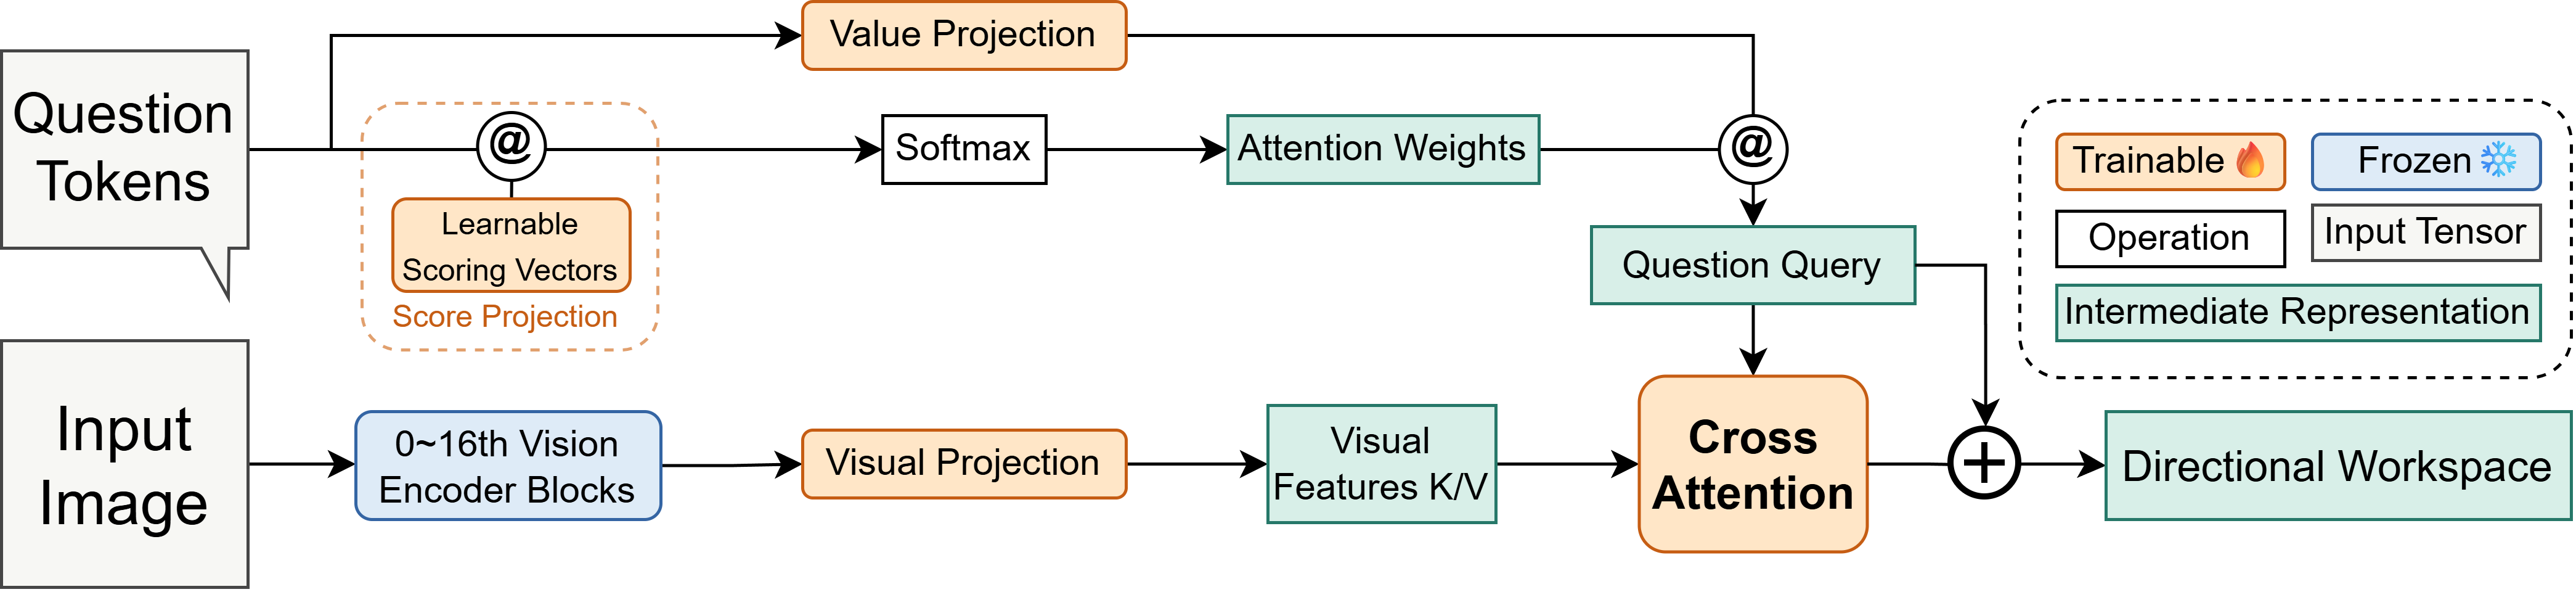
\includegraphics[width=\textwidth]{figures/directional_workspace.png}
    \caption{Directional Workspace的构造。问题Token嵌入经可训练评分向量和Value Projection形成Query；第17层之前的视觉Token投影为K/V。Cross-Attention读取与问题相关的视觉证据，并通过残差连接得到聚合表示。视觉Block采用从0开始的编号，K/V取自索引0至16的Block输出。}
    \label{fig:directional-workspace}
\end{figure}

视觉K/V取自同一样本在第17个视觉Block入口处的图像Token $H^{v}$。通过可训练投影
$W_k,W_v\in\mathbb{R}^{d_v\times D}$得到

\begin{equation}
K=H^{v}W_k,\qquad V=H^{v}W_v.
\end{equation}

以问题表示检索图像区域是视觉问答中的常见建模方式\cite{Anderson2017BottomUpAT,Kim2018BilinearAN}。QDPT采用16头Cross-Attention\cite{Vaswani2017AttentionIA}，以问题表示为Query、图像表示为K/V：

\begin{align}
O &= \operatorname{MHA}(Q,K,V),\\
Z &= Q+O,
\end{align}

其中$Z\in\mathbb{R}^{m\times D}$即Directional Workspace。宽度$D$控制问题投影、视觉投影和跨模态注意力的容量。默认设置为$D=768$。

“Directional”指两种模态在注意力中的固定角色：问题Token形成Query，图像Token只作为K/V。输出$Z$用于生成语言Prompt，不参与视觉编码器后续各层的计算。

\begin{figure}[t]
    \centering
    \begingroup
    \setlength{\unitlength}{\textwidth}
    \begin{picture}(1,0.31187)
        \put(0,0){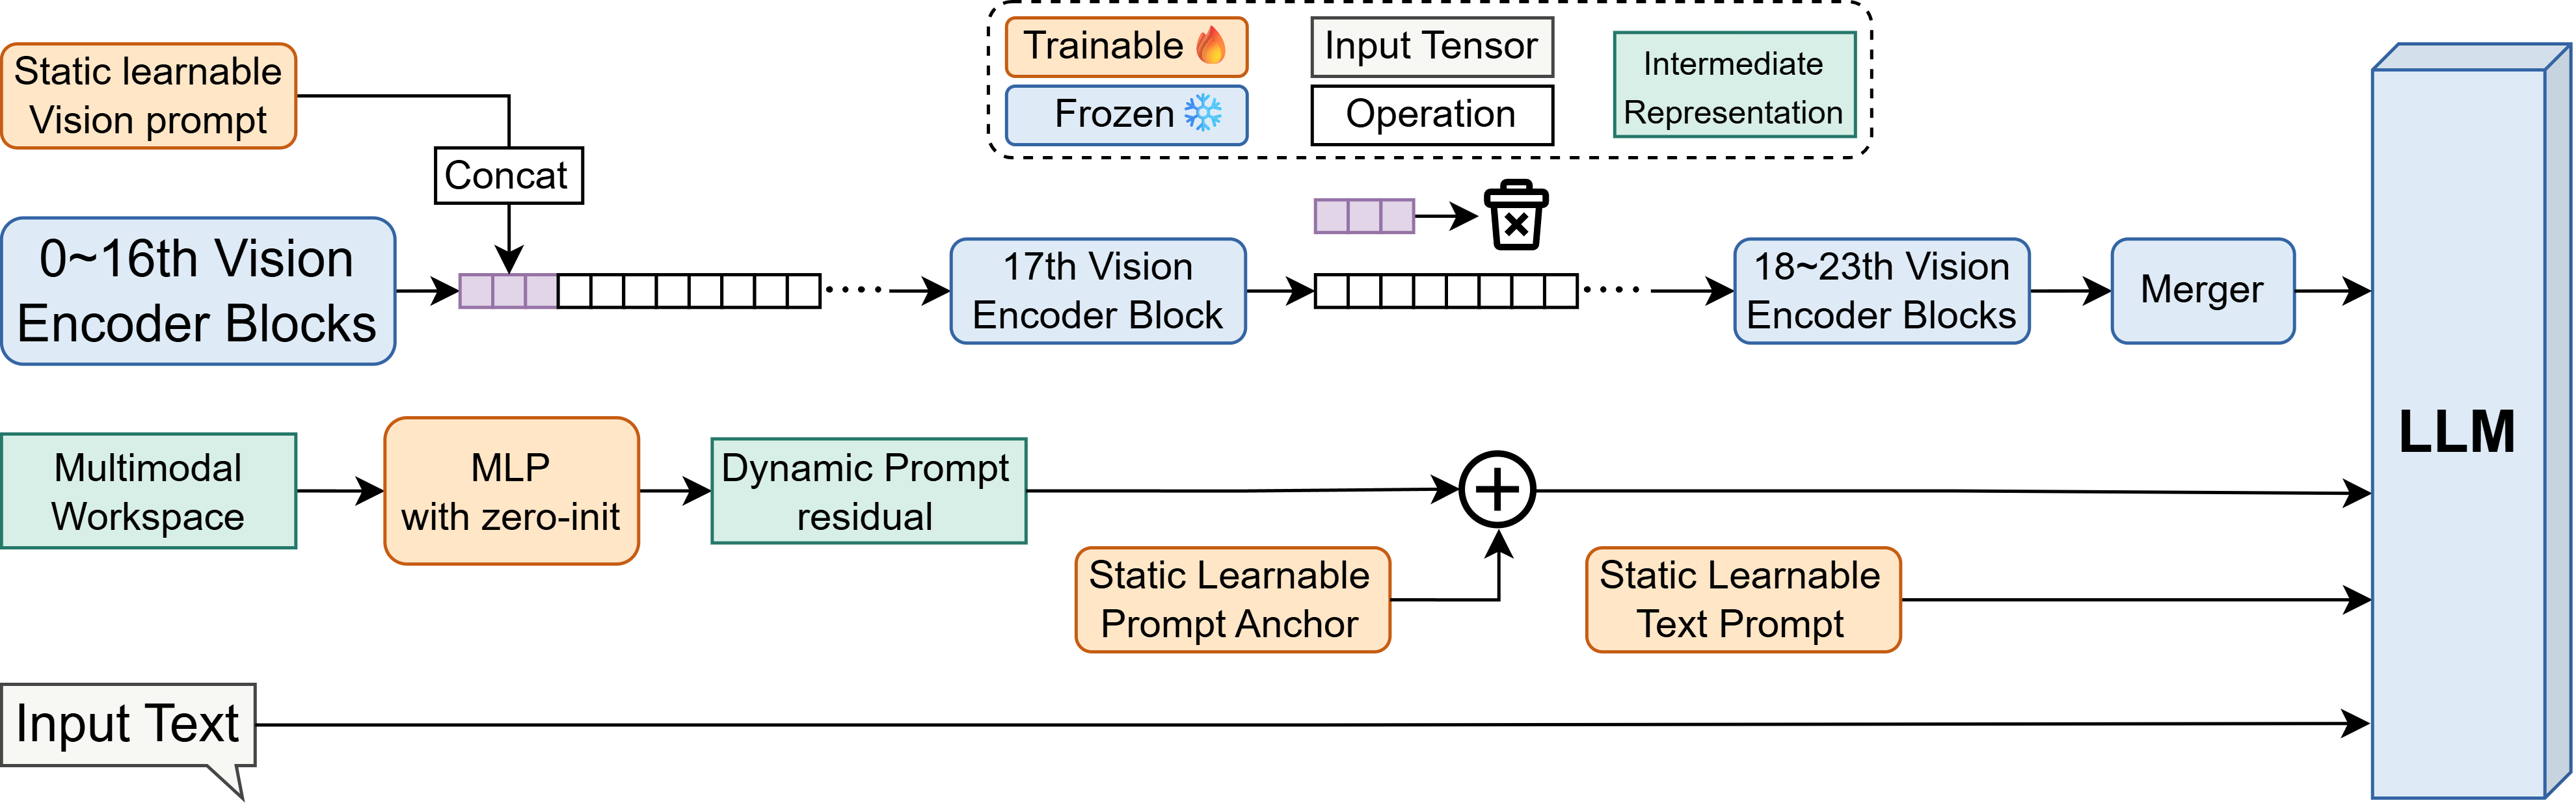
\includegraphics[width=\textwidth]{figures/qdpt_overview.png}}
        \put(0.002,0.099){\color[RGB]{218,239,233}\rule{0.111\textwidth}{0.042\textwidth}}
        \put(0.0575,0.120){\makebox(0,0){\sffamily\resizebox{0.096\textwidth}{!}{\shortstack{Directional\\Workspace}}}}
    \end{picture}
    \endgroup
    \caption{视觉主路径与动态Prompt输出路径。本图承接图\ref{fig:directional-workspace}生成的Workspace。静态视觉Prompt在第17个视觉Block中提供领域校准，并在该层之后移除；问题条件的Directional Workspace只读取视觉证据，经语言侧映射生成动态Prompt。各路输入在LLM入口的排列见图\ref{fig:causal-placement}。视觉Block采用从0开始的编号，第17个Block指索引17。}
    \label{fig:qdpt-overview}
\end{figure}

图\ref{fig:qdpt-overview}承接图\ref{fig:directional-workspace}的聚合结果，展示动态Prompt的生成及其与视觉主路径的衔接。

Directional Workspace通过映射函数
$g_{\theta}:\mathbb{R}^{D}\rightarrow\mathbb{R}^{d_l}$
逐槽转换为语言侧残差：

\begin{equation}
\begin{aligned}
\Delta P^{d}&=g_{\theta}(Z),\\
g_{\theta}(Z)&=\operatorname{GELU}\!\left(\operatorname{LN}(Z)W_1+b_1\right)W_2+b_2.
\end{aligned}
\end{equation}

其中$W_1\in\mathbb{R}^{768\times768}$、$W_2\in\mathbb{R}^{768\times2560}$，映射逐槽执行，两个线性层均含偏置，GELU使用tanh近似。参考零初始化适配器的做法\cite{Zhang2023LLaMAAdapterEF}，输出层的权重与偏置在训练开始时置零，因此初始动态残差为零。模型另维护10个静态可训练Anchor
$A^{t}\in\mathbb{R}^{m\times d_l}$，最终动态Prompt为

\begin{equation}
P^{d}=A^{t}+\Delta P^{d}.
\end{equation}

训练开始时$P^{d}=A^{t}$，随后输出映射逐步学习样本相关的残差。

推理时，动态分支执行问题池化、视觉Cross-Attention和Prompt映射，不针对测试样本进行反向传播。

\subsection{因果输入排列与参数规模}

自回归LLM中的Token顺序会改变各类Prompt能够影响的后续表示。QDPT采用图\ref{fig:causal-placement}所示的输入顺序：静态领域Prompt位于视觉Token之前，问题条件的动态Prompt位于视觉Token之后、问题Token之前。对应的输入序列为

\begin{equation}
E_{\mathrm{LLM}}
= [P^{t};M(I);P^{d};T(X)].
\end{equation}

\begin{figure}[t]
    \centering
    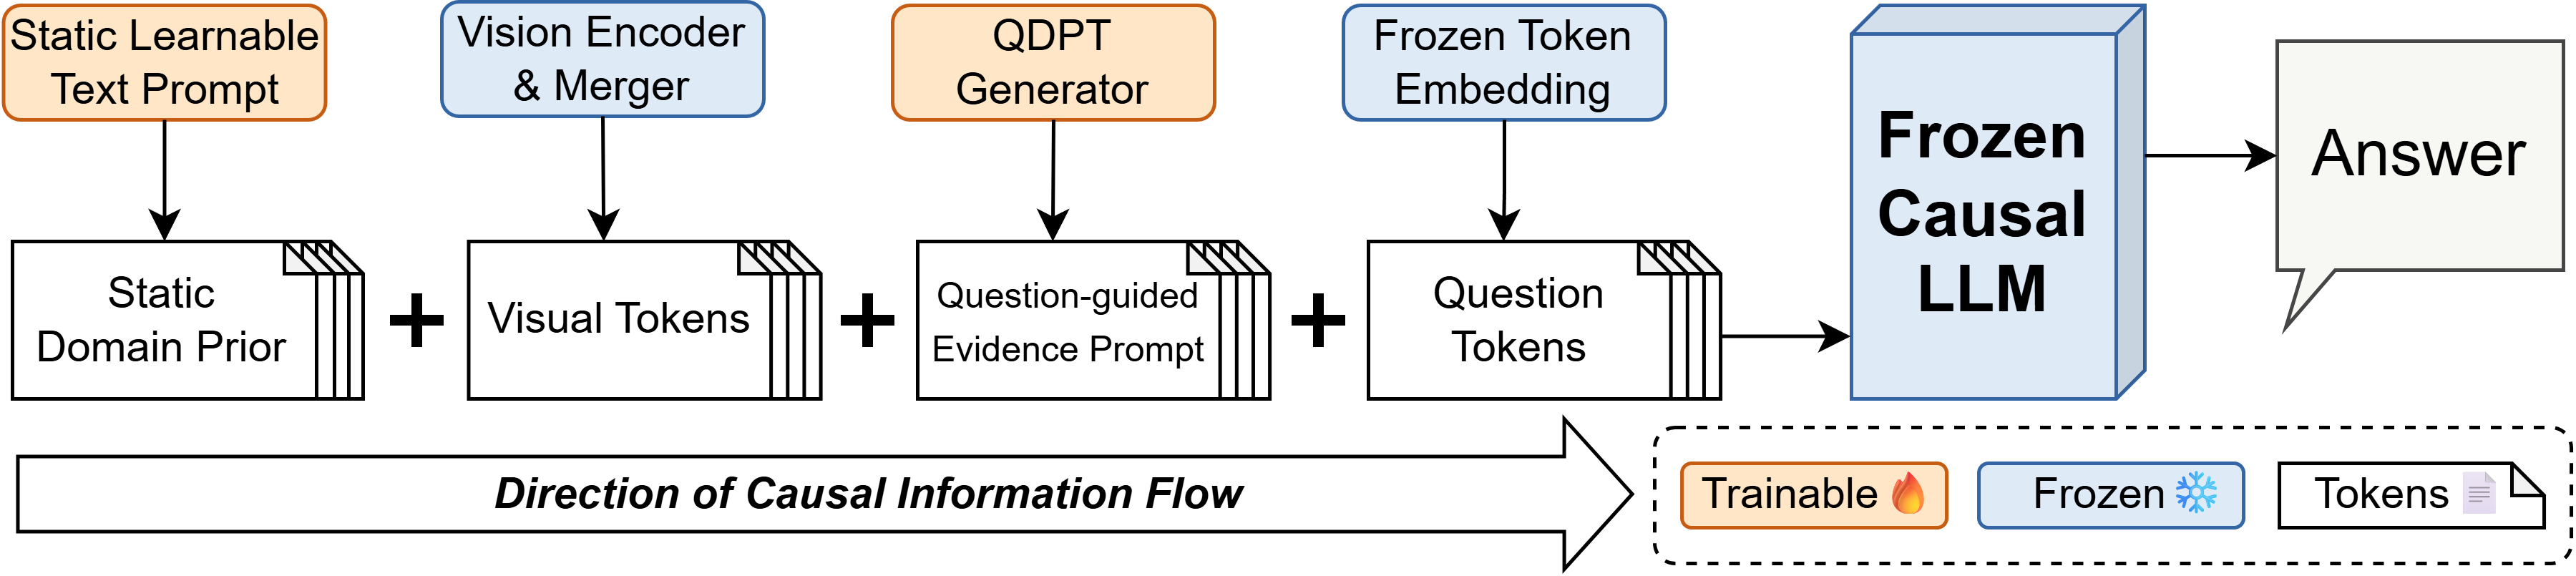
\includegraphics[width=\textwidth]{figures/causal_prompt_placement.png}
    \caption{QDPT在冻结因果LLM中的Prompt放置。静态Prompt位于视觉Token之前，用作领域先验；问题引导的证据Prompt位于视觉Token之后并紧邻问题。箭头表示由因果掩码决定的前向可见方向。}
    \label{fig:causal-placement}
\end{figure}

按照这一顺序，视觉Token能够访问前置的静态Prompt，问题及答案Token能够访问两类Prompt和视觉表示。本文在模型、训练协议和Prompt数量不变的条件下比较其他排列，结果见实验部分。

QDPT共有7,805,184个可训练参数，具体组成见表\ref{tab:trainable-params}。静态语言Prompt、动态Prompt Anchor和静态视觉Prompt合计95,232个参数，占适配器的1.22\%；其余7,709,952个参数用于问题池化、视觉K/V投影、16头Cross-Attention和动态Prompt输出头。

\begin{table}[t]
    \centering
    \caption{QDPT的可训练参数组成。}
    \label{tab:trainable-params}
    \begin{tabular}{lrr}
        \toprule
        模块 & 配置 & 参数量 \\
        \midrule
        静态语言Prompt $P^{t}$ & $20\times2560$ & 51,200 \\
        动态Prompt Anchor $A^{t}$ & $10\times2560$ & 25,600 \\
        静态视觉Prompt $P^{v}$ & $18\times1024$ & 18,432 \\
        问题池化、跨模态检索与输出头 & $D=768$ & 7,709,952 \\
        \midrule
        合计 &  & 7,805,184 \\
        \bottomrule
    \end{tabular}
\end{table}

动态生成器的参数量主要由适配宽度和输出映射决定。输出头压缩的容量对照见附录\ref{sec:output-head-appendix}。训练时，冻结层仍参与前向计算及适配器所需的梯度回传，计算成本还取决于适配参数在骨干中的位置。

\section{实验}

本章在同一冻结骨干和评价脚本下比较QDPT、静态Prompt、实例条件Prompt与LoRA，并分析Prompt输入位置、训练效率与随机种子稳定性。

\subsection{实验设置}

\subsubsection{数据集}

视觉问答要求模型根据图像和自然语言问题生成答案\cite{Agrawal2015VQAVQ}。PathVQA\cite{He2020PathVQA3Q}是主要开发数据集。结构选择在官方Validation划分上完成，Test划分仅用于最终配置的评估。本文同时报告Overall、Yes/No和Free-form准确率，以区分封闭式判断与开放式生成。

SLAKE\cite{Liu2021SlakeAS}用于检查同一结构在另一数据集上的表现。两个公开数据集使用相同的QDPT结构配置。除Overall外，实验还统计CLOSED与OPEN、KVQA与VQA，以及英文和中文问题。

自建电力电气数据集由本实验室采购的电力设备图像及目标检测标注整理而成。训练集包含20,015张图像，并借助Gemma 3 27B IT将检测标签、类别、目标数量和场景信息转换为36,700条多模态指令，任务包括设备与部件识别、缺陷与异常判断。固定测试集包含972张训练集之外的图像，每张图像对应一道经过人工核对的选择题。其中18个样本因图像文件关联缺失被排除，所有方法均在相同的954个有效样本上计算准确率。该数据集不公开。

\subsubsection{比较方法}

所有方法使用同一Qwen3-VL骨干\cite{Bai2025Qwen3VLTR}、图像预处理和答案评估脚本。Static LLM Prompt、Static Visual Prompt与Dual Static Prompt分别在语言侧、视觉侧或两侧加入样本共享的连续Prompt\cite{lester2021power,jia2022visual}。CoCoOp-style是CoCoOp\cite{Zhou2022ConditionalPL}在生成式MLLM上的近似复现：保留图像条件Meta-Net与共享连续上下文，用Merger输出的图像Token均值生成条件偏置，并将其加到语言Prompt上。Full-Attention LoRA-r8\cite{Hu2022LoRA}在视觉编码器和语言模型的全部注意力层加入秩为8的低秩更新，作为权重空间适配参照。GRASP\cite{Sun2026GRASPGR}没有可用的官方代码，独立实现及核验过程移至附录\ref{sec:grasp-appendix}，不参与主表排序。

\subsubsection{训练与评价协议}

实验使用单张NVIDIA GeForce RTX 5090，软件环境为PyTorch 2.8.0、torchvision 0.23.0和Transformers 5.0.0；PyTorch与torchvision均为CUDA 12.8构建，驱动支持CUDA 13.0。所有方法使用BF16精度并冻结原始骨干参数，仅优化新增适配参数。输入采用Qwen3-VL原始AutoProcessor的动态分辨率策略，各方法均未额外指定固定图像分辨率或视觉Token上限，文本序列最大长度为2048。

QDPT使用AdamW，$\beta_1=0.9$、$\beta_2=0.999$、$\epsilon=10^{-8}$，所有参数组的权重衰减为0。学习率在前3\%训练步内线性预热，随后线性衰减；梯度范数裁剪阈值为1.0，不使用梯度检查点。训练共3个epoch，单卡微批量为2，梯度累积16步，有效batch size为32。20个静态语言Prompt $P^t$与10个文本Anchor $A^t$的学习率为0.3。18个静态视觉Prompt分为两组：前8个使用$3\times10^{-5}$，其余10个使用$10^{-4}$；问题池化、视觉投影、跨注意力与输出映射均使用$10^{-4}$。

Full-Attention LoRA采用$r=8$、$\alpha=16$和0.05的dropout，不训练偏置，不使用DoRA。其更新覆盖24层视觉自注意力的融合qkv及输出proj，以及36层语言自注意力的q、k、v、o投影，共192个线性层，包含7,077,888个可训练参数。LoRA同样使用AdamW、零权重衰减、3\%预热和线性衰减，学习率为$10^{-4}$，微批量为1、梯度累积32步。Static LLM Prompt使用20个宽度为2560的Token，共51,200个参数，学习率为0.3。CoCoOp-style使用20个Prompt Token和隐藏宽度为160的条件网络，共873,120个可训练参数，Prompt与条件网络的学习率分别为0.3和$3\times10^{-4}$。

模型结构和超参数在PathVQA Validation上确定，此后用于多随机种子实验、SLAKE及电气数据集。主实验均使用第3个epoch的检查点。公开基准的多次运行使用模型种子44、45、46，单次对照使用44；数据采样种子固定为42。SLAKE只沿用PathVQA确定的结构和超参数，适配器直接在SLAKE训练集上重新训练。各方法共享数据划分、输入模板和评价程序。公开VQA指标为答案归一化后的Exact Match准确率，电气选择题按解析后的选项与标准答案匹配计分。评估采用贪心解码，temperature设为0，最多生成32个Token。三次运行报告均值$\pm$样本标准差，单次运行直接报告准确率，表中列明种子数。

对于逐样本配对比较，差值统一定义为对照或消融模型的准确率减去完整模型的准确率。图像聚类Bootstrap按图像有放回重采样，每次保留该图像对应的全部问题，共重复10,000次；95\%置信区间取差值分布的2.5\%和97.5\%百分位数。McNemar检验采用双侧精确二项检验，不作连续性校正。

\subsection{PathVQA结果}

表\ref{tab:pathvqa-main}汇总PathVQA Validation结果。最终QDPT的三随机种子平均Overall为59.15，与LoRA-r8的59.26相差0.11个百分点。QDPT高于Static LLM Prompt和CoCoOp-style，但其标准差也更大。单次运行中，Static Visual Prompt的Free-form准确率为3.29；同时在视觉侧和语言侧加入静态Prompt后，Dual Static Prompt的Overall升至54.63。

\begin{table}[t]
    \centering
    \caption{PathVQA Validation上的受控比较（\%）。三次运行报告均值$\pm$标准差，其他方法报告单次结果。}
    \label{tab:pathvqa-main}
    \scriptsize
    \setlength{\tabcolsep}{2pt}
    \begin{tabular}{@{}lrrrrr@{}}
        \toprule
        方法 & 参数量 & 种子数 & Overall & Yes/No & Free-form \\
        \midrule
        Static Visual Prompt & 0.020M & 1 & 35.95 & 68.70 & 3.29 \\
        Dual Static Prompt & 0.072M & 1 & 54.63 & 88.38 & 20.96 \\
        Static LLM Prompt & 0.051M & 3 & $55.08\pm0.22$ & $88.95\pm0.55$ & $21.30\pm0.91$ \\
        CoCoOp-style & 0.873M & 3 & $56.31\pm1.14$ & $89.35\pm0.59$ & $23.37\pm1.69$ \\
        QDPT & 7.805M & 3 & $59.15\pm1.75$ & $91.65\pm1.03$ & $26.75\pm2.51$ \\
        \midrule
        Full-Attention LoRA-r8 & 7.078M & 3 & $59.26\pm0.07$ & $91.72\pm0.41$ & $26.90\pm0.28$ \\
        \bottomrule
    \end{tabular}
\end{table}

结构确定后，各方法使用第3个epoch的检查点评估PathVQA Test，结果见表\ref{tab:pathvqa-test}。QDPT的三随机种子平均Overall为58.88，较Static LLM Prompt和CoCoOp-style分别高2.80和1.93个百分点；LoRA-r8为59.66，比QDPT高0.78个百分点。所有检查点均在Validation阶段确定，未根据Test结果重新选择配置。

\begin{table}[t]
    \centering
    \caption{PathVQA Test Overall结果（\%）。多次运行报告均值$\pm$标准差。}
    \label{tab:pathvqa-test}
    \scriptsize
    \begin{tabular}{@{}lrr@{}}
        \toprule
        方法 & 种子数 & Overall \\
        \midrule
        Frozen Base & 1 & 34.77 \\
        Static LLM Prompt & 3 & $56.08\pm0.36$ \\
        CoCoOp-style & 3 & $56.95\pm0.84$ \\
        QDPT & 3 & $58.88\pm1.81$ \\
        Full-Attention LoRA-r8 & 3 & $59.66\pm0.02$ \\
        \bottomrule
    \end{tabular}
\end{table}

QDPT在Test上的Yes/No与Free-form准确率分别为$91.32\pm1.15$和$26.39\pm2.49$。开放题的运行间波动更大，后文结合Validation结果讨论这一现象。

\subsection{SLAKE结果}

QDPT沿用在PathVQA上确定的结构和超参数，在SLAKE训练集上重新训练适配器。表\ref{tab:slake-results}给出Test结果。QDPT的平均Overall为76.95，比Static LLM Prompt高2.55个百分点，在OPEN、VQA及中英文子集上也取得更高准确率。LoRA-r8达到81.82，比QDPT高4.87个百分点，并在各项拆分上保持优势。差距主要集中在知识型问答和开放式回答：QDPT在KVQA上为62.17，较LoRA低8.24个百分点，在OPEN上低6.12个百分点，而CLOSED上的差距为2.99个百分点。

与静态语言Prompt相比，QDPT在VQA上提高2.97个百分点，但KVQA从62.55降至62.17，说明当前结构对知识型问答的适配不足。QDPT通过10个动态输入Prompt调整语言模型的上下文，LoRA则直接更新视觉与语言注意力变换。两者适配位置和参数作用方式的差异，可能与知识型问答及开放回答上的表现差距有关。这些子集结果还不能将误差定位到视觉提取、知识调用或答案生成中的某一个环节。

英文与中文子集上，QDPT分别落后5.34和4.39个百分点。差距同时出现在两种语言中，后续改进需要关注知识型问题和开放回答，而非仅调整某一种语言的输出形式。

\begin{table}[t]
    \centering
    \caption{SLAKE Test结果（\%）。三次运行报告均值$\pm$标准差。}
    \label{tab:slake-results}
    \scriptsize
    \begin{tabular}{@{}lrrrr@{}}
        \toprule
        方法 & 种子数 & Overall & CLOSED & OPEN \\
        \midrule
        Static LLM Prompt & 1 & 74.40 & 80.62 & 70.27 \\
        QDPT & 3 & $76.95\pm0.44$ & $84.01\pm1.32$ & $72.26\pm1.14$ \\
        Full-Attention LoRA-r8 & 3 & $81.82\pm0.22$ & $87.00\pm0.39$ & $78.38\pm0.62$ \\
        \bottomrule
    \end{tabular}
    \par\smallskip
    \begin{tabular}{@{}lrrrr@{}}
        \toprule
        方法 & KVQA & VQA & EN & ZH \\
        \midrule
        Static LLM Prompt & 62.55 & 76.14 & 75.40 & 73.38 \\
        QDPT & $62.17\pm0.00$ & $79.11\pm0.51$ & $77.51\pm1.44$ & $76.38\pm0.64$ \\
        Full-Attention LoRA-r8 & $70.41\pm1.72$ & $83.49\pm0.08$ & $82.85\pm0.41$ & $80.77\pm0.05$ \\
        \bottomrule
    \end{tabular}
\end{table}

\subsection{电力电气数据集结果}

表\ref{tab:electrical-results}报告相同954个有效样本上的准确率。QDPT答对681题，在本次单种子实验中取得71.38\%的最高准确率；Full-Attention LoRA-r8答对677题，两者相差4题。这组结果构成设备图像问答上的应用验证。

\begin{table}[t]
    \centering
    \caption{自建电力电气数据集固定留出集结果（\%）。每种方法均为单次运行，共954条有效预测。}
    \label{tab:electrical-results}
    \small
    \begin{tabular}{@{}lrr@{}}
        \toprule
        方法 & 可训练参数 & Overall \\
        \midrule
        Static LLM Prompt & 51,200 & 69.50 \\
        CoCoOp-style & 873,120 & 70.34 \\
        Full-Attention LoRA-r8 & 7,077,888 & 70.96 \\
        QDPT & 7,805,184 & 71.38 \\
        \bottomrule
    \end{tabular}
\end{table}

\subsection{适配宽度选择}

在确定LLM侧Prompt位置之前，我们固定其余模块和训练协议，仅改变Directional Workspace的宽度$D$。表\ref{tab:workspace-width}给出seed 44的Validation结果。$D=1024$的Overall为59.58\%，$D=768$为59.56\%，两者相差0.02个百分点；逐样本McNemar检验为$p=1.0$，图像聚类Bootstrap的差值95\%置信区间为$[-0.76,0.74]$。$D=768$使用7.805M参数，比$D=1024$少26.54\%，Free-form准确率高0.48个百分点。

宽度降至512后，Overall较768低0.88个百分点，配对差值95\%置信区间为$[-1.60,-0.13]$；$D=256$在Yes/No和Free-form上进一步下降。在该次实验中，$D=768$与$D=1024$的准确率接近，而前者参数更少，因此后续实验采用$D=768$。

\begin{table}[htbp]
    \centering
    \caption{PathVQA Validation上的Directional Workspace宽度比较（seed 44，\%）。各配置采用相同的输入顺序$[P^{t};P^{d};M(I);T(X)]$。}
    \label{tab:workspace-width}
    \small
    \begin{tabular}{@{}rrrrr@{}}
        \toprule
        宽度$D$ & 可训练参数 & Overall & Yes/No & Free-form \\
        \midrule
        256  & 2.033M  & 57.15 & 89.47 & 24.92 \\
        512  & 4.592M  & 58.68 & 90.85 & 26.61 \\
        768  & 7.805M  & 59.56 & 91.04 & 28.17 \\
        1024 & 10.626M & 59.58 & 91.55 & 27.70 \\
        \bottomrule
    \end{tabular}
\end{table}

\subsection{问题引导与视觉读取消融}

机制消融包含两组参照。最终配置的输入顺序记为
\begin{equation}
    \mathcal{S}_{f}=[P^{t};M(I);P^{d};T(X)],
\end{equation}
位置定型前使用的顺序记为
\begin{equation}
    \mathcal{S}_{o}=[P^{t};P^{d};M(I);T(X)].
\end{equation}
两组实验只在各自顺序内比较，不交叉计算差值。

Learned Query对照采用$\mathcal{S}_{f}$，保留视觉K/V、Cross-Attention、Prompt位置和训练设置。它以可学习表$Q_s\in\mathbb{R}^{10\times2560}$替代问题池化中的评分矩阵，并沿用实际参与前向与优化的问题投影$W_q$：
\begin{equation}
    Q_{\mathrm{learned}}=\operatorname{LN}_q(Q_s)W_q.
\end{equation}
$Q_s$采用均值为0、标准差为0.02的正态分布初始化。$\operatorname{LN}_q$与问题条件分支复用同一归一化层，含可训练仿射参数，其缩放和偏置分别初始化为1和0。替换前后的可训练张量均参与计算，两个完整模型各含7,805,184个可训练参数；该设计匹配可训练参数量，但不假定两种Query具有完全相同的表达能力。在这三次运行中，问题条件Query的平均准确率高出0.83个百分点，但优势未在所有种子中复现。

其余两项消融采用$\mathcal{S}_{o}$，参照模型的Overall为59.56\%。关闭动态分支的视觉读取，即令$Z=Q$，准确率降至57.63\%；消融模型与完整模型的独有正确样本数分别为237和358，McNemar检验$p=7.98\times10^{-7}$，图像聚类Bootstrap的差值95\%置信区间为$[-2.76,-1.10]$。移除18个静态视觉Prompt后，准确率为58.44\%，两侧独有正确样本数为261和331，$p=0.00453$，差值95\%置信区间为$[-1.89,-0.35]$。原图和原问题仍通过Qwen3-VL主路径；这两项实验只改变QDPT新增支路。

\begin{table}[t]
    \centering
    \caption{PathVQA Validation上的机制消融（\%）。同一输入顺序内采用相同训练设置。}
    \label{tab:mechanism-ablation}
    \scriptsize
    \setlength{\tabcolsep}{2pt}
    \begin{tabular}{@{}llrrrr@{}}
        \toprule
        配置 & 输入顺序 & 参数量 & Seed 44 & Seed 45 & Seed 46 \\
        \midrule
        QDPT & $\mathcal{S}_{f}$ & 7.805M & 60.78 & 57.29 & 59.39 \\
        Learned Query & $\mathcal{S}_{f}$ & 7.805M & 59.05 & 57.72 & 58.19 \\
        \midrule
        QDPT & $\mathcal{S}_{o}$ & 7.805M & 59.56 & --- & --- \\
        $Z=Q$ & $\mathcal{S}_{o}$ & 7.805M$^{*}$ & 57.63 & --- & --- \\
        去除静态视觉Prompt & $\mathcal{S}_{o}$ & 7.787M & 58.44 & --- & --- \\
        \bottomrule
    \end{tabular}
    \par\smallskip
    \raggedright\footnotesize $^{*}$Cross-Attention参数只为保持初始化与检查点结构一致而保留，不参与该对照的前向输出或梯度更新。
\end{table}

\subsection{Prompt放置位置消融}

因果LLM只能访问当前位置之前的Token，因此Prompt排列会改变信息传播路径。表\ref{tab:prompt-placement}固定模型、参数量和训练协议，只调整输入顺序，并分别运行seed 44、45和46。QDPT采用的顺序在seed 44上领先另外两种排列1.52和2.65个百分点，但seed 45中两种对照均反超1.12个百分点。三随机种子均值相差0.19和0.61个百分点，远小于QDPT自身1.75的标准差。由此可见，输入位置会改变优化结果，但当前实验没有得到跨初始化一致的最优排列。最终顺序是在seed 44 Validation上预先选定的，后续Test和SLAKE实验保持该配置不变。

\begin{table}[t]
    \centering
    \caption{PathVQA Validation上的Prompt放置位置消融（\%）。三种配置均含7,805,184个可训练参数，表中为三随机种子及其均值$\pm$标准差。}
    \label{tab:prompt-placement}
    \scriptsize
    \begin{tabular}{@{}lrrrr@{}}
        \toprule
        输入顺序 & Seed 44 & Seed 45 & Seed 46 & Mean $\pm$ SD \\
        \midrule
        $[P^{t};M(I);P^{d};T(X)]$（QDPT） & 60.78 & 57.29 & 59.39 & $59.15\pm1.75$ \\
        $[M(I);P^{t};P^{d};T(X)]$ & 59.26 & 58.41 & 59.23 & $58.97\pm0.48$ \\
        $[P^{d};M(I);P^{t};T(X)]$ & 58.12 & 58.41 & 59.10 & $58.55\pm0.50$ \\
        \bottomrule
    \end{tabular}
\end{table}

\subsection{训练效率}

表\ref{tab:training-efficiency}给出PathVQA训练集上的受控吞吐测试。QDPT和LoRA-r8均采用微批量1、梯度累积32步、单进程数据加载，在相同的数据顺序上先预热20个优化器步，再连续计时100步。计时开始前执行CUDA同步并重置峰值显存统计，结束时再次同步；连续窗口包含训练循环中的数据准备、前向、反向和参数更新，不包含评估或检查点写入。两个窗口各处理3200个样本和1,202,879个Merger输出视觉Token。QDPT达到7.30 samples/s，是LoRA-r8的1.88倍；峰值分配显存为15.81 GiB，比LoRA-r8低3.51 GiB。

\begin{table}[t]
    \centering
    \caption{PathVQA训练集上使用RTX 5090完成的受控训练吞吐测试。两种方法采用相同微批量、梯度累积、样本序列和视觉Token数量。}
    \label{tab:training-efficiency}
    \small
    \begin{tabular}{@{}lrrr@{}}
        \toprule
        方法 & 100步时间（s） & samples/s & 峰值分配（GiB） \\
        \midrule
        QDPT & 438.07 & 7.30 & 15.81 \\
        Full-Attention LoRA-r8 & 824.08 & 3.88 & 19.32 \\
        \bottomrule
    \end{tabular}
\end{table}

\subsection{随机种子稳定性}

图\ref{fig:seed-stability}给出PathVQA Validation上的三随机种子结果。LoRA-r8的标准差为0.07，Static LLM Prompt为0.22；CoCoOp-style和QDPT分别为1.14与1.75。容量匹配的Learned Query标准差为0.67。QDPT三次运行的范围达到3.48个百分点，运行间差异大于本实验中的其他方法。

\begin{figure}[t]
    \centering
    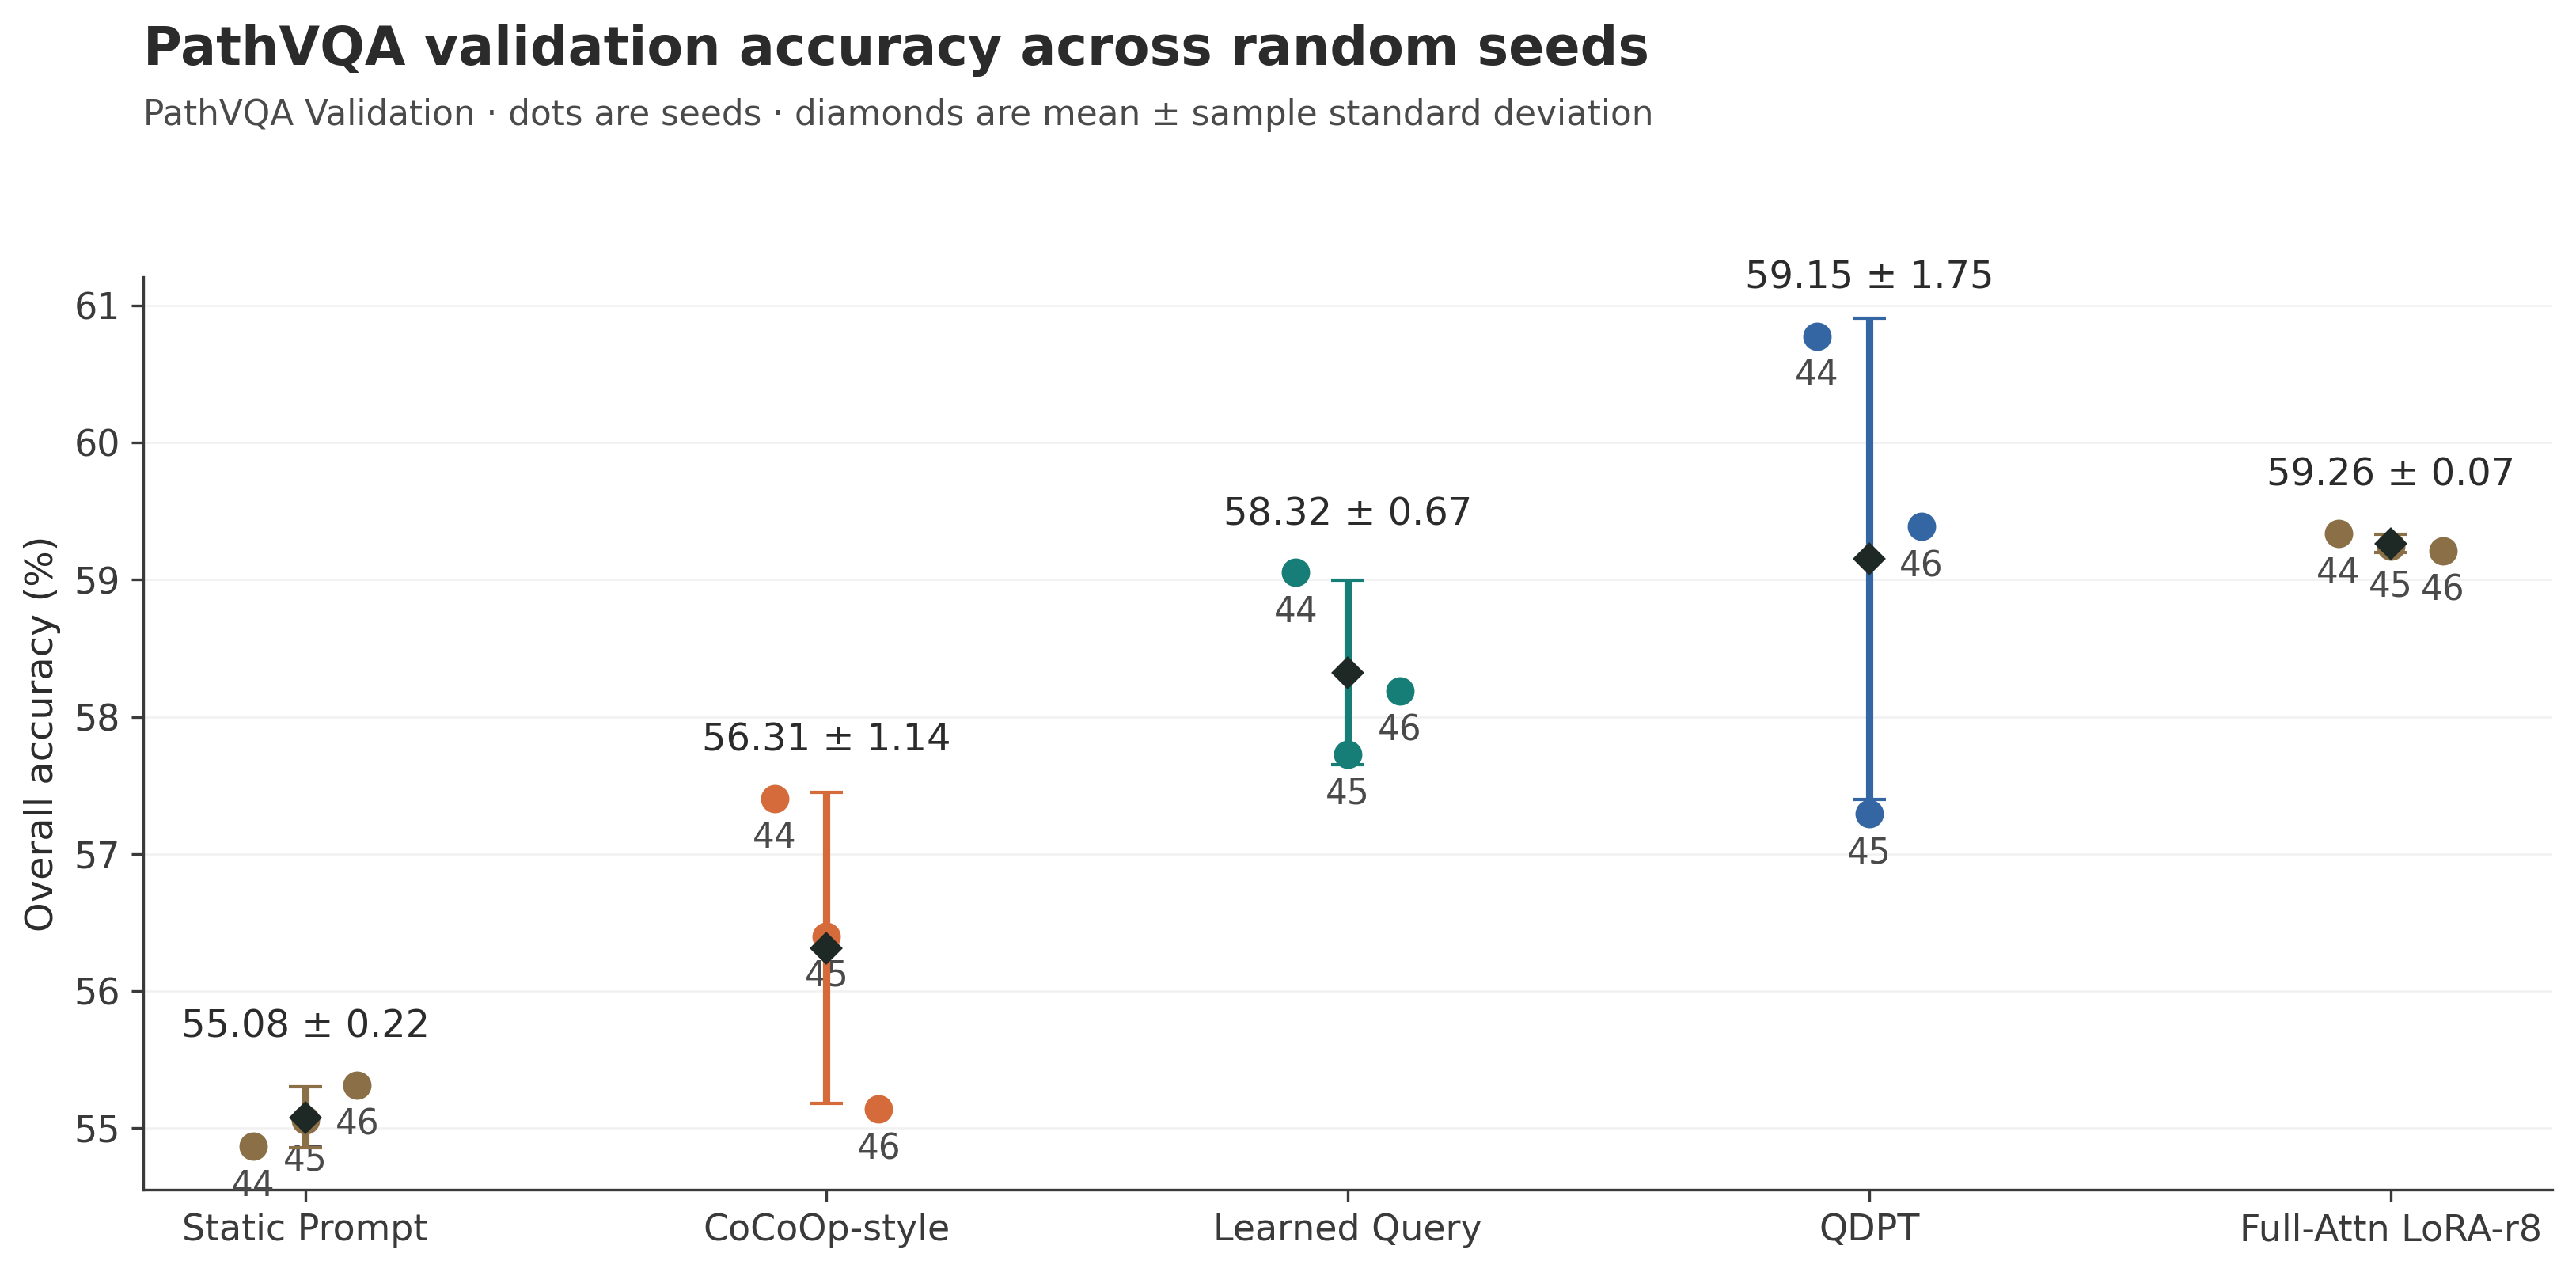
\includegraphics[width=\textwidth,trim=0 0 0 42bp,clip]{figures/pathvqa_seed_stability.png}
    \caption{PathVQA Validation Overall的三随机种子分布。圆点表示单次运行，菱形和误差线表示均值与样本标准差。}
    \label{fig:seed-stability}
\end{figure}

\subsection{结果讨论}

QDPT在PathVQA Validation上与LoRA取得接近的平均准确率，在SLAKE上则落后4.87个百分点。电气实验中，QDPT比LoRA多答对4题，这组单次结果用于设备图像上的应用验证。SLAKE的分项差距更有解释价值：QDPT在KVQA和OPEN上分别落后8.24和6.12个百分点，说明当前Prompt接口对知识型问题和开放回答的适配仍然不足。

机制消融分别检验问题条件化和视觉读取。采用$\mathcal{S}_{f}$时，问题条件Query的三次运行均值比可训练参数量相同的Learned Query高0.83个百分点，但seed 45出现反转。采用$\mathcal{S}_{o}$时，关闭动态分支的视觉读取使准确率由59.56\%降至57.63\%，移除静态视觉Prompt后为58.44\%。后两项的配对检验和图像聚类Bootstrap支持观察到的单次运行差值。

位置实验呈现出另一种现象。seed 44支持当前排列，seed 45却出现反转，三种排列的均值差也明显小于QDPT自身的运行波动。位置会影响训练轨迹，但优势方向依赖初始化。因此，当前输入顺序应视为Validation阶段固定下来的实现选择，不承担核心机制证据。

QDPT有7.805M可训练参数，约占4.445B骨干的0.18\%，略多于LoRA的7.078M。在统一微批量、样本序列和视觉Token数量的短程测试中，QDPT的训练吞吐为LoRA的1.88倍，峰值分配显存低18.18\%。这项差异来自当前两种适配实现的完整训练路径，尚未拆分到具体算子。附录中的输出头压缩减少了参数量，却带来3.36个百分点的准确率损失，没有改善本次实验的精度与容量折中。

训练稳定性仍是QDPT的不足。PathVQA上，QDPT三次运行的标准差为1.75，高于静态Prompt的0.22和CoCoOp-style的1.14。Test上的Free-form标准差为2.49，也高于Yes/No的1.15。较大的运行间差异可能与动态生成器的联合优化有关，现有诊断尚未定位主要来源。问题池化对固定Token集合的排列不敏感，也限制了动态分支对词序关系的表达。后续可分别考察问题编码方式和生成器优化设置，以改善关系表达与训练稳定性。

\section{结论}

本文提出QDPT，通过问题Token池化与视觉Cross-Attention生成语言侧动态Prompt，用于冻结多模态大模型的领域适配。在Qwen3-VL-4B-Instruct上，QDPT使用约7.81M可训练参数，PathVQA Test准确率达到58.88\%，较静态语言Prompt提高2.80个百分点。问题条件Query在三次参数量匹配对照中平均高于Learned Query 0.83个百分点，但优势随随机种子变化；关闭视觉读取或移除静态视觉Prompt也会降低准确率。统一条件下的短程测试测得1.88倍于LoRA-r8的训练吞吐。电气选择题结果补充了设备图像上的应用验证。SLAKE的知识型问答与开放回答、PathVQA的运行稳定性仍是QDPT的主要不足。后续工作将改进问题分支的词序表达，并降低动态生成器对初始化的敏感性。


\appendix
\section{动态Prompt输出头容量对照}
\label{sec:output-head-appendix}

输出头压缩实验保留$D=768$的Workspace，并将动态Prompt输出头改为秩256的低秩映射。表\ref{tab:output-head}显示，该改动减少21.84\%的可训练参数，同时使Overall下降3.36个百分点，Free-form下降4.76个百分点。该压缩配置未达到预期的精度与参数量折中，因此主实验采用默认输出头。该对照考察的是固定适配宽度下的一种输出瓶颈设置。

\begin{table}[t]
    \centering
    \caption{PathVQA Validation上的动态Prompt输出头容量对照（seed 44，\%）。}
    \label{tab:output-head}
    \small
    \begin{tabular}{@{}lrrrr@{}}
        \toprule
        配置 & 可训练参数 & Overall & Yes/No & Free-form \\
        \midrule
        QDPT（默认输出头） & 7,805,184 & 60.78 & 92.74 & 28.91 \\
        QDPT（秩256输出头） & 6,100,736 & 57.42 & 90.78 & 24.15 \\
        \bottomrule
    \end{tabular}
\end{table}

\section{GRASP独立实现结果}
\label{sec:grasp-appendix}

GRASP在实验开展时没有可用的官方代码。我们依据论文描述完成独立实现，并观察了Prompt初始化和二维位置编码对结果的影响，见表\ref{tab:grasp-appendix}。这些配置采用本文统一的三轮训练协议，与原论文的任务和训练预算不同，因此作为实现核验记录置于附录，不参与主表排序。

\begin{table}[t]
    \centering
    \caption{GRASP独立实现的PathVQA Validation结果（seed 44，\%）。}
    \label{tab:grasp-appendix}
    \small
    \begin{tabular}{@{}lrrr@{}}
        \toprule
        配置 & Overall & Yes/No & Free-form \\
        \midrule
        统一三轮独立实现 & 39.75 & 75.36 & 4.24 \\
        Qwen初始化与分组学习率 & 42.40 & 76.22 & 8.68 \\
        去除固定二维位置编码 & 43.92 & 79.04 & 8.90 \\
        \bottomrule
    \end{tabular}
\end{table}

\section{训练过程诊断}
\label{sec:training-diagnostics-appendix}

图\ref{fig:training-dynamics}记录QDPT在PathVQA上的三次完整训练。三条日志损失曲线接近，但Prompt范数、Workspace表示尺度和视觉注意力熵在训练中逐渐分离。该现象与最终准确率的运行间差异同时出现，不过这些轨迹不能单独确定差异来自哪个模块。

\begin{figure}[htbp]
    \centering
    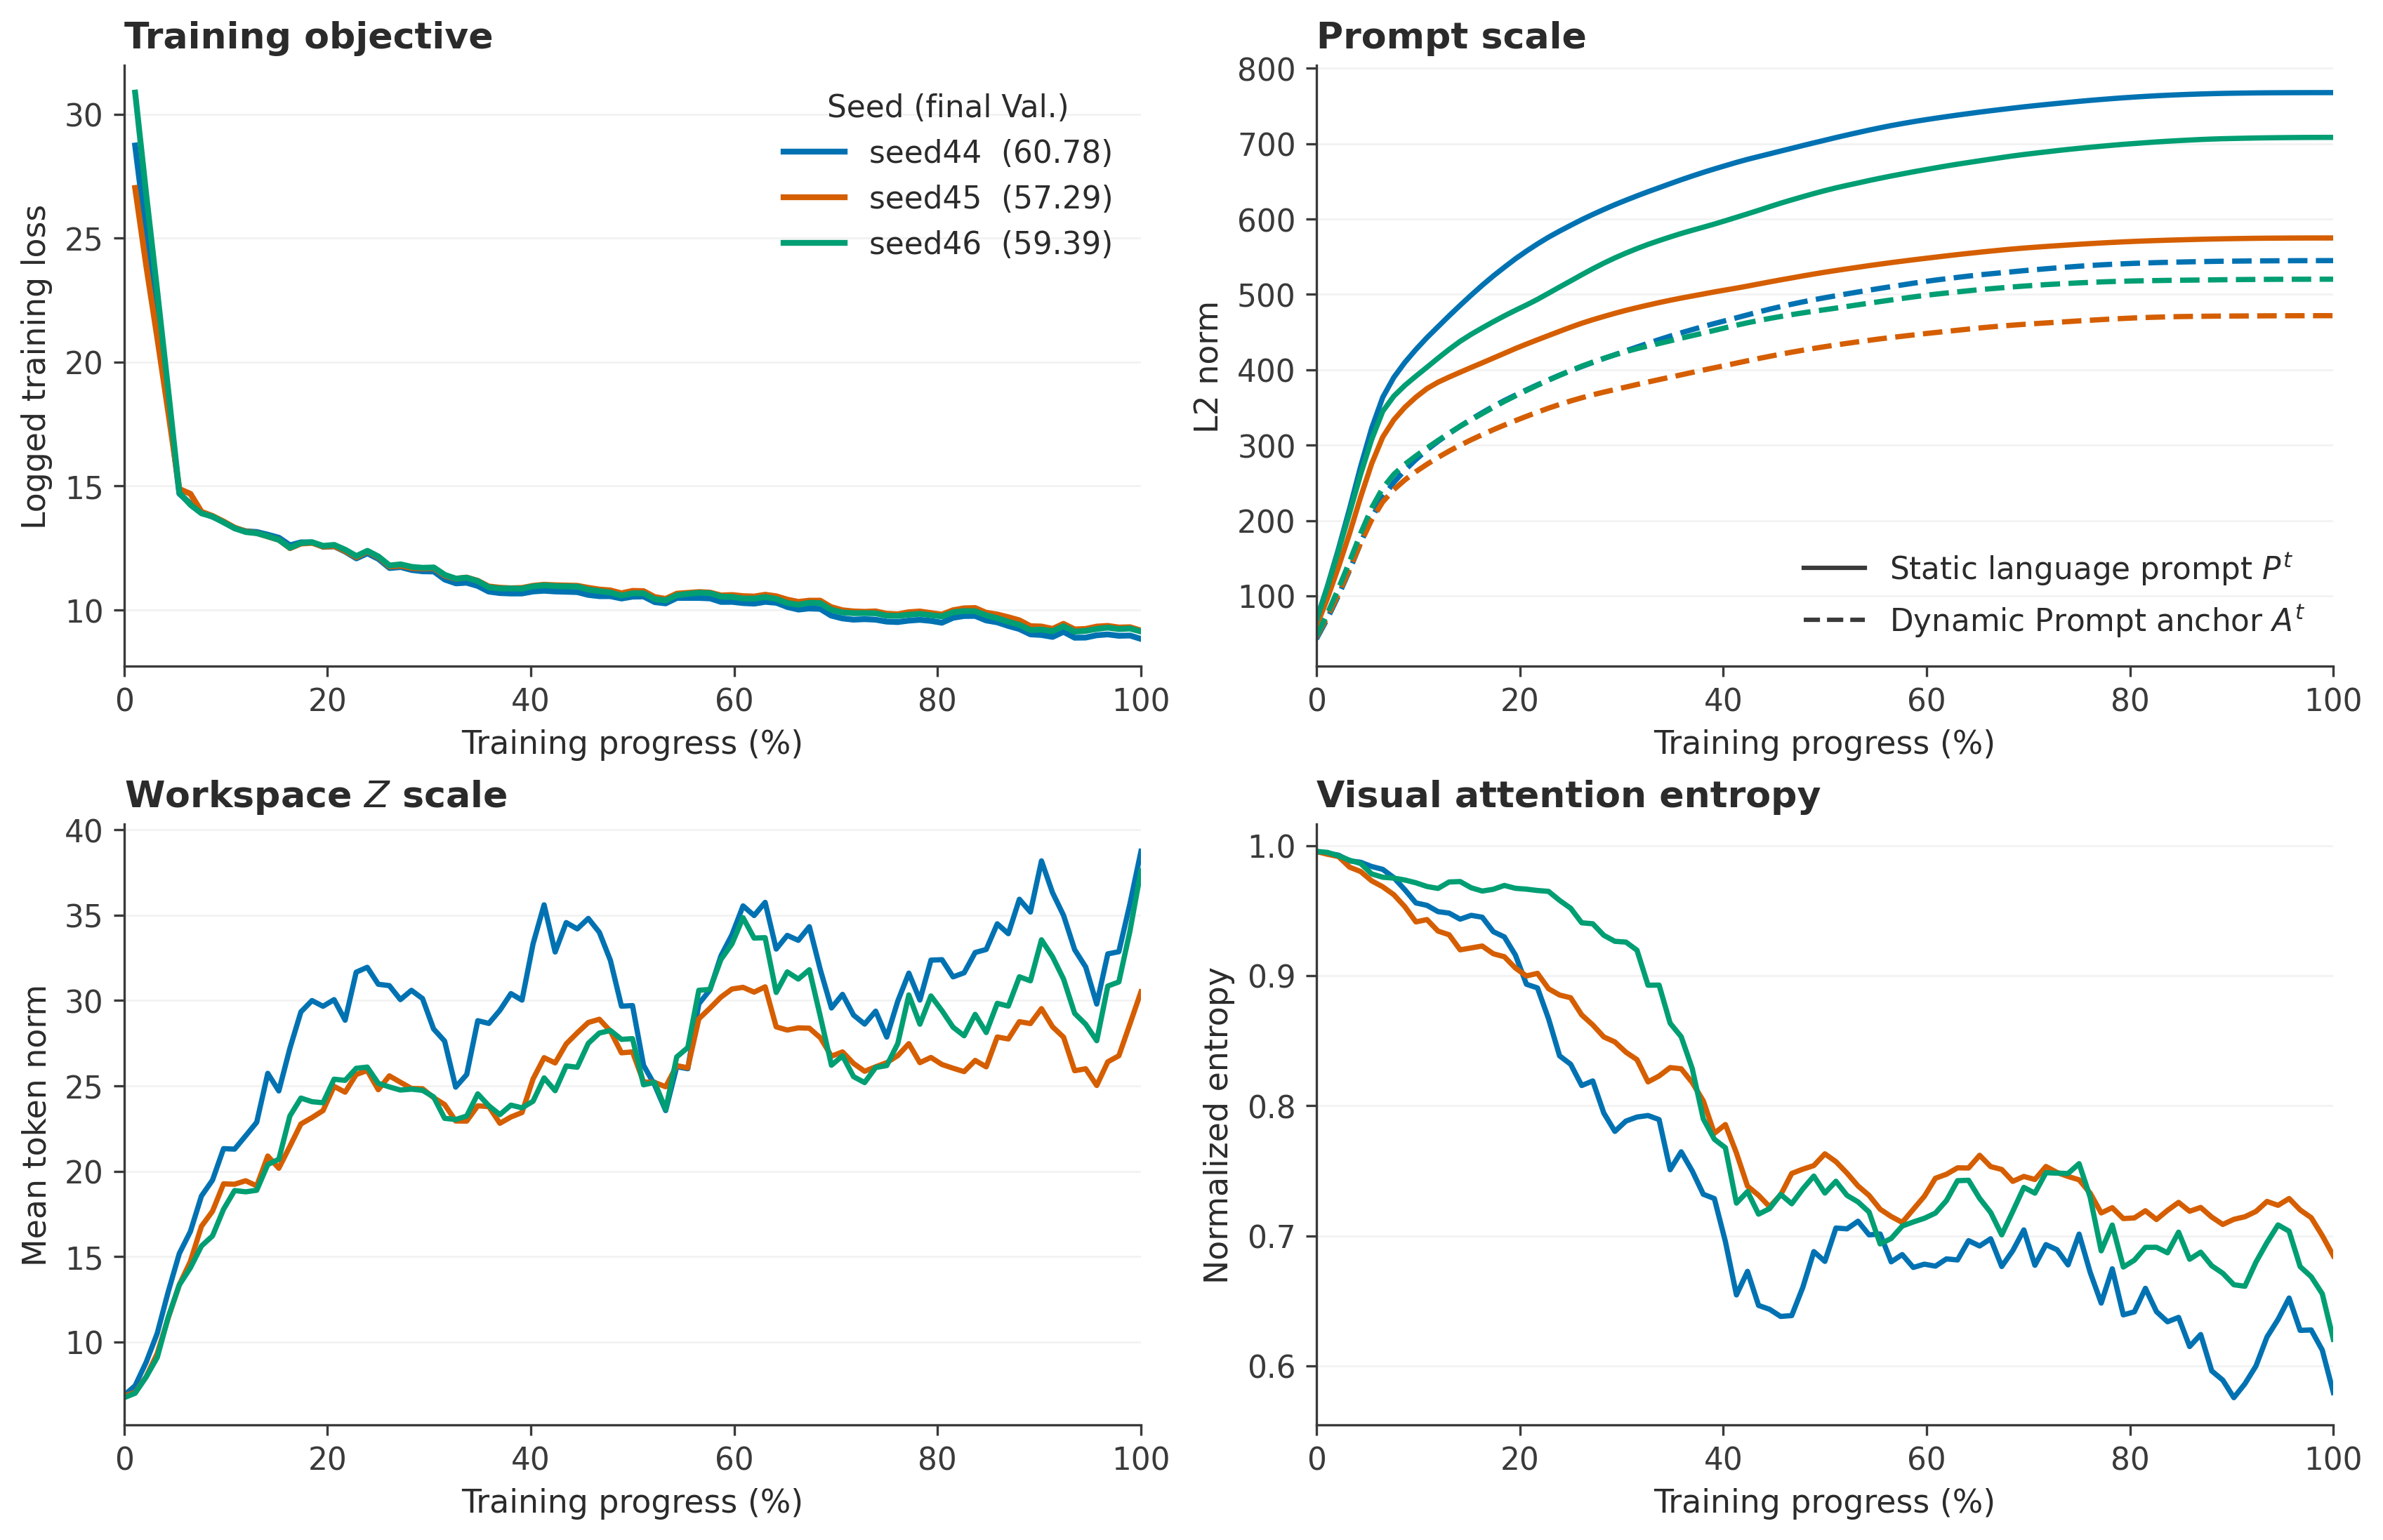
\includegraphics[width=\textwidth]{figures/qdpt_training_dynamics.png}
    \caption{QDPT在PathVQA上的三随机种子训练轨迹。训练器每20个优化器步记录一次区间平均损失，图中各曲线采用7点滑动平均；横轴按各次运行的记录步数归一化。右上图的实线与虚线分别表示静态语言Prompt $P^t$和文本Anchor的$L_2$范数。视觉注意力熵先以有效视觉Token数的对数归一化，再对batch、注意力头和Query槽取平均。}
    \label{fig:training-dynamics}
\end{figure}


\backmatter

\section*{Data availability}
PathVQA and SLAKE are publicly available from their respective providers. The private electrical inspection dataset is not publicly available.
% 待补：Funding、Competing interests、Code availability、Author contributions。

\bibliography{qdpt-references}

\end{document}
